%% bare_conf.tex
%% V1.4b
%% 2015/08/26
%% by Michael Shell
%% See:
%% http://www.michaelshell.org/
%% for current contact information.
%%
%% This is a skeleton file demonstrating the use of IEEEtran.cls
%% (requires IEEEtran.cls version 1.8b or later) with an IEEE
%% conference paper.
%%
%% Support sites:
%% http://www.michaelshell.org/tex/ieeetran/
%% http://www.ctan.org/pkg/ieeetran
%% and
%% http://www.ieee.org/

%%*************************************************************************
%% Legal Notice:
%% This code is offered as-is without any warranty either expressed or
%% implied; without even the implied warranty of MERCHANTABILITY or
%% FITNESS FOR A PARTICULAR PURPOSE! 
%% User assumes all risk.
%% In no event shall the IEEE or any contributor to this code be liable for
%% any damages or losses, including, but not limited to, incidental,
%% consequential, or any other damages, resulting from the use or misuse
%% of any information contained here.
%%
%% All comments are the opinions of their respective authors and are not
%% necessarily endorsed by the IEEE.
%%
%% This work is distributed under the LaTeX Project Public License (LPPL)
%% ( http://www.latex-project.org/ ) version 1.3, and may be freely used,
%% distributed and modified. A copy of the LPPL, version 1.3, is included
%% in the base LaTeX documentation of all distributions of LaTeX released
%% 2003/12/01 or later.
%% Retain all contribution notices and credits.
%% ** Modified files should be clearly indicated as such, including  **
%% ** renaming them and changing author support contact information. **
%%*************************************************************************

% *** Authors should verify (and, if needed, correct) their LaTeX system  ***
% *** with the testflow diagnostic prior to trusting their LaTeX platform ***
% *** with production work. The IEEE's font choices and paper sizes can   ***
% *** trigger bugs that do not appear when using other class files.       ***                          ***
% The testflow support page is at:
% http://www.michaelshell.org/tex/testflow/

\documentclass[conference]{IEEEtran}
% Some Computer Society conferences also require the compsoc mode option,
% but others use the standard conference format.
%
% If IEEEtran.cls has not been installed into the LaTeX system files,
% manually specify the path to it like:
% \documentclass[conference]{../sty/IEEEtran}

% Some very useful LaTeX packages include:
% (uncomment the ones you want to load)

% *** MISC UTILITY PACKAGES ***
%
%\usepackage{ifpdf}
% Heiko Oberdiek's ifpdf.sty is very useful if you need conditional
% compilation based on whether the output is pdf or dvi.
% usage:
% \ifpdf
%   % pdf code
% \else
%   % dvi code
% \fi
% The latest version of ifpdf.sty can be obtained from:
% http://www.ctan.org/pkg/ifpdf
% Also, note that IEEEtran.cls V1.7 and later provides a builtin
% \ifCLASSINFOpdf conditional that works the same way.
% When switching from latex to pdflatex and vice-versa, the compiler may
% have to be run twice to clear warning/error messages.

% *** CITATION PACKAGES ***
%
%\usepackage{cite}
% cite.sty was written by Donald Arseneau
% V1.6 and later of IEEEtran pre-defines the format of the cite.sty package
% \cite{} output to follow that of the IEEE. Loading the cite package will
% result in citation numbers being automatically sorted and properly
% "compressed/ranged". e.g., [1], [9], [2], [7], [5], [6] without using
% cite.sty will become [1], [2], [5]--[7], [9] using cite.sty. cite.sty's
% \cite will automatically add leading space, if needed. Use cite.sty's
% noadjust option (cite.sty V3.8 and later) if you want to turn this off
% such as if a citation ever needs to be enclosed in parenthesis.
% cite.sty is already installed on most LaTeX systems. Be sure and use
% version 5.0 (2009-03-20) and later if using hyperref.sty.
% The latest version can be obtained at:
% http://www.ctan.org/pkg/cite
% The documentation is contained in the cite.sty file itself.

% *** GRAPHICS RELATED PACKAGES ***
%
\ifCLASSINFOpdf
   \usepackage[pdftex]{graphicx}
  % declare the path(s) where your graphic files are
  % \graphicspath{{../pdf/}{../jpeg/}}
  % and their extensions so you won't have to specify these with
  % every instance of \includegraphics
  % \DeclareGraphicsExtensions{.pdf,.jpeg,.png}
\else
  % or other class option (dvipsone, dvipdf, if not using dvips). graphicx
  % will default to the driver specified in the system graphics.cfg if no
  % driver is specified.
  % \usepackage[dvips]{graphicx}
  % declare the path(s) where your graphic files are
  % \graphicspath{{../eps/}}
  % and their extensions so you won't have to specify these with
  % every instance of \includegraphics
  % \DeclareGraphicsExtensions{.eps}
\fi
% graphicx was written by David Carlisle and Sebastian Rahtz. It is
% required if you want graphics, photos, etc. graphicx.sty is already
% installed on most LaTeX systems. The latest version and documentation
% can be obtained at: 
% http://www.ctan.org/pkg/graphicx
% Another good source of documentation is "Using Imported Graphics in
% LaTeX2e" by Keith Reckdahl which can be found at:
% http://www.ctan.org/pkg/epslatex
%
% latex, and pdflatex in dvi mode, support graphics in encapsulated
% postscript (.eps) format. pdflatex in pdf mode supports graphics
% in .pdf, .jpeg, .png and .mps (metapost) formats. Users should ensure
% that all non-photo figures use a vector format (.eps, .pdf, .mps) and
% not a bitmapped formats (.jpeg, .png). The IEEE frowns on bitmapped formats
% which can result in "jaggedy"/blurry rendering of lines and letters as
% well as large increases in file sizes.
%
% You can find documentation about the pdfTeX application at:
% http://www.tug.org/applications/pdftex

% *** MATH PACKAGES ***
%
\usepackage{amsmath}
% A popular package from the American Mathematical Society that provides
% many useful and powerful commands for dealing with mathematics.
%
% Note that the amsmath package sets \interdisplaylinepenalty to 10000
% thus preventing page breaks from occurring within multiline equations. Use:
%\interdisplaylinepenalty=2500
% after loading amsmath to restore such page breaks as IEEEtran.cls normally
% does. amsmath.sty is already installed on most LaTeX systems. The latest
% version and documentation can be obtained at:
% http://www.ctan.org/pkg/amsmath

% *** SPECIALIZED LIST PACKAGES ***
%
%\usepackage{algorithmic}
% algorithmic.sty was written by Peter Williams and Rogerio Brito.
% This package provides an algorithmic environment fo describing algorithms.
% You can use the algorithmic environment in-text or within a figure
% environment to provide for a floating algorithm. Do NOT use the algorithm
% floating environment provided by algorithm.sty (by the same authors) or
% algorithm2e.sty (by Christophe Fiorio) as the IEEE does not use dedicated
% algorithm float types and packages that provide these will not provide
% correct IEEE style captions. The latest version and documentation of
% algorithmic.sty can be obtained at:
% http://www.ctan.org/pkg/algorithms
% Also of interest may be the (relatively newer and more customizable)
% algorithmicx.sty package by Szasz Janos:
% http://www.ctan.org/pkg/algorithmicx

% *** ALIGNMENT PACKAGES ***
%
%\usepackage{array}
% Frank Mittelbach's and David Carlisle's array.sty patches and improves
% the standard LaTeX2e array and tabular environments to provide better
% appearance and additional user controls. As the default LaTeX2e table
% generation code is lacking to the point of almost being broken with
% respect to the quality of the end results, all users are strongly
% advised to use an enhanced (at the very least that provided by array.sty)
% set of table tools. array.sty is already installed on most systems. The
% latest version and documentation can be obtained at:
% http://www.ctan.org/pkg/array

% IEEEtran contains the IEEEeqnarray family of commands that can be used to
% generate multiline equations as well as matrices, tables, etc., of high
% quality.

% *** SUBFIGURE PACKAGES ***
%\ifCLASSOPTIONcompsoc
%  \usepackage[caption=false,font=normalsize,labelfont=sf,textfont=sf]{subfig}
%\else
%  \usepackage[caption=false,font=footnotesize]{subfig}
%\fi
% subfig.sty, written by Steven Douglas Cochran, is the modern replacement
% for subfigure.sty, the latter of which is no longer maintained and is
% incompatible with some LaTeX packages including fixltx2e. However,
% subfig.sty requires and automatically loads Axel Sommerfeldt's caption.sty
% which will override IEEEtran.cls' handling of captions and this will result
% in non-IEEE style figure/table captions. To prevent this problem, be sure
% and invoke subfig.sty's "caption=false" package option (available since
% subfig.sty version 1.3, 2005/06/28) as this is will preserve IEEEtran.cls
% handling of captions.
% Note that the Computer Society format requires a larger sans serif font
% than the serif footnote size font used in traditional IEEE formatting
% and thus the need to invoke different subfig.sty package options depending
% on whether compsoc mode has been enabled.
%
% The latest version and documentation of subfig.sty can be obtained at:
% http://www.ctan.org/pkg/subfig

% *** FLOAT PACKAGES ***
%
%\usepackage{fixltx2e}
% fixltx2e, the successor to the earlier fix2col.sty, was written by
% Frank Mittelbach and David Carlisle. This package corrects a few problems
% in the LaTeX2e kernel, the most notable of which is that in current
% LaTeX2e releases, the ordering of single and double column floats is not
% guaranteed to be preserved. Thus, an unpatched LaTeX2e can allow a
% single column figure to be placed prior to an earlier double column
% figure.
% Be aware that LaTeX2e kernels dated 2015 and later have fixltx2e.sty's
% corrections already built into the system in which case a warning will
% be issued if an attempt is made to load fixltx2e.sty as it is no longer
% needed.
% The latest version and documentation can be found at:
% http://www.ctan.org/pkg/fixltx2e

%\usepackage{stfloats}
% stfloats.sty was written by Sigitas Tolusis. This package gives LaTeX2e
% the ability to do double column floats at the bottom of the page as well
% as the top. (e.g., "\begin{figure*}[!b]" is not normally possible in
% LaTeX2e). It also provides a command:
%\fnbelowfloat
% to enable the placement of footnotes below bottom floats (the standard
% LaTeX2e kernel puts them above bottom floats). This is an invasive package
% which rewrites many portions of the LaTeX2e float routines. It may not work
% with other packages that modify the LaTeX2e float routines. The latest
% version and documentation can be obtained at:
% http://www.ctan.org/pkg/stfloats
% Do not use the stfloats baselinefloat ability as the IEEE does not allow
% \baselineskip to stretch. Authors submitting work to the IEEE should note
% that the IEEE rarely uses double column equations and that authors should try
% to avoid such use. Do not be tempted to use the cuted.sty or midfloat.sty
% packages (also by Sigitas Tolusis) as the IEEE does not format its papers in
% such ways.
% Do not attempt to use stfloats with fixltx2e as they are incompatible.
% Instead, use Morten Hogholm'a dblfloatfix which combines the features
% of both fixltx2e and stfloats:
%
% \usepackage{dblfloatfix}
% The latest version can be found at:
% http://www.ctan.org/pkg/dblfloatfix

% *** PDF, URL AND HYPERLINK PACKAGES ***
%
%\usepackage{url}
% url.sty was written by Donald Arseneau. It provides better support for
% handling and breaking URLs. url.sty is already installed on most LaTeX
% systems. The latest version and documentation can be obtained at:
% http://www.ctan.org/pkg/url
% Basically, \url{my_url_here}.

% *** Do not adjust lengths that control margins, column widths, etc. ***
% *** Do not use packages that alter fonts (such as pslatex).         ***
% There should be no need to do such things with IEEEtran.cls V1.6 and later.
% (Unless specifically asked to do so by the journal or conference you plan
% to submit to, of course. )

% correct bad hyphenation here
\hyphenation{op-tical net-works semi-conduc-tor}

\begin{document}
%
% paper title
% Titles are generally capitalized except for words such as a, an, and, as,
% at, but, by, for, in, nor, of, on, or, the, to and up, which are usually
% not capitalized unless they are the first or last word of the title.
% Linebreaks \\ can be used within to get better formatting as desired.
% Do not put math or special symbols in the title.
\title{Carry-Free Implementations of Arithmetic Operations in FPGA}


% author names and affiliations
% use a multiple column layout for up to three different
% affiliations
\author{\IEEEauthorblockN{Vikram Voleti}
\IEEEauthorblockA{International Institute of Information Technology, Hyderabad\\
Email: vikram.voleti@gmail.com}}

% conference papers do not typically use \thanks and this command
% is locked out in conference mode. If really needed, such as for
% the acknowledgment of grants, issue a \IEEEoverridecommandlockouts
% after \documentclass

% for over three affiliations, or if they all won't fit within the width
% of the page, use this alternative format:
% 
%\author{\IEEEauthorblockN{Michael Shell\IEEEauthorrefmark{1},
%Homer Simpson\IEEEauthorrefmark{2},
%James Kirk\IEEEauthorrefmark{3}, 
%Montgomery Scott\IEEEauthorrefmark{3} and
%Eldon Tyrell\IEEEauthorrefmark{4}}
%\IEEEauthorblockA{\IEEEauthorrefmark{1}School of Electrical and Computer Engineering\\
%Georgia Institute of Technology,
%Atlanta, Georgia 30332--0250\\ Email: see http://www.michaelshell.org/contact.html}
%\IEEEauthorblockA{\IEEEauthorrefmark{2}Twentieth Century Fox, Springfield, USA\\
%Email: homer@thesimpsons.com}
%\IEEEauthorblockA{\IEEEauthorrefmark{3}Starfleet Academy, San Francisco, California 96678-2391\\
%Telephone: (800) 555--1212, Fax: (888) 555--1212}
%\IEEEauthorblockA{\IEEEauthorrefmark{4}Tyrell Inc., 123 Replicant Street, Los Angeles, California 90210--4321}}

% use for special paper notices
%\IEEEspecialpapernotice{(Invited Paper)}

% make the title area
\maketitle

% As a general rule, do not put math, special symbols or citations
% in the abstract
\begin{abstract}
This paper uses Recoded Binary Signed Digits to perform carry-free arithmetic operations of addition, subtraction and (Karatsuba) multiplication on binary numbers. Detailed truth tables and logic circuits of the carry-free implementation of addition are provided. Detailed circuit design of carry-free multiplication is also drawn. We compare the path delays and FPGA utilizations with that of standard implementation. The problem of implementing carry-free arithmetic is analyzed, and design improvements to our method are provided.
\end{abstract}

% no keywords

% For peer review papers, you can put extra information on the cover
% page as needed:
% \ifCLASSOPTIONpeerreview
% \begin{center} \bfseries EDICS Category: 3-BBND \end{center}
% \fi
%
% For peerreview papers, this IEEEtran command inserts a page break and
% creates the second title. It will be ignored for other modes.
\IEEEpeerreviewmaketitle


\section{Introduction}

Even with recent development in technology of integrated circuits, various high-speed circuits with regular structures and low power design still suffer from problems of path delay, limited range of the number of bits, and complexity in hardware. It is well-known that the addition of radix-$B$ numbers suffers from carry propagation. Since the speed of digital processors depends mostly on the speed of the adders used in the system, it is critical to optimize the addition operation to speed up all computations.

Simple carry-ripple adders take time proportional to the length of the longest path from input to output. Even though this can be reduced to a depth of $O(log(n))$ by carry-lookahead adders [1], the depth still grows with the number of digits, and cannot be improved upon unless a different number system is used. Signed digit number systems [2-8] could be used to eliminate carry propagation and perform addition in $O(1)$ time. However, as [8] explains, the standard addition algorithms do not work for binary numbers ($B$ = 2).

[9, 10] suggest to recode the input numbers so that subsequent addition and subtraction of binary numbers become carry-free. Parhami [9], in particular, recodes the numbers into a format that allows carry-free arithmetic operations effectively. In this paper, this format is used to recode binary numbers for carry-free arithmetic operations (see section IV). Since the focus is on using carry-free logic to perform arithmetic operations on binary numbers, the goal is to make arithmetic modules that take binary numbers as input, and perform addition or multiplication on them. To consider least memory requirement, only the minimal digit set {-1, 0, 1} has been considered. It is also of significant advantage to have these circuits as reusable modules in building circuits for more complex arithmetic operations, like modular reduction, which has significant relevance in cryptographic applications.

In this paper, circuits for the addition of the recoded numbers, addition of binary numbers in a non-naive way, and multiplication of binary numbers have been designed. The modular nature of these circuits is exemplified by the use of Carry-Free Adders as modules to build the Carry-Free Multiplier. These circuits have been implemented on an FPGA, and their speeds and area requirements have been compared with those of standard addition. The carry-free implementations are then analyzed to probe their limitations and suggest remedies for future work.

The contents of this paper are: (i) details of the conversion between binary, signed digit, and Recoded Binary Signed Digit (see section IV) numbers, with truth table and logic equations, (ii) implementation of arithmetic operations of addition, subtraction, multiplication using carry-free logic (sections V, VI), (iii) comparison of the carry-free implementations and their standard versions (section VII), (iv) analysis of the carry-free implementations (section VIII).


\section{Related Work}

[11] begins to design a carry-free multiplier. This paper details all the design features involved to create an end-to-end carry-free multiplier using carry-free adders as modules. [12] uses the same digit format as us, that mentioned in [9], but uses trinary signed digits. [13] uses bit-pair recording to generate partial products, and then adds them in the form of a binary tree using a carry-free adder. This paper's carry-free multiplier uses the Karatsuba multiplication algorithm [14] (see section VI) and performs all additions using a carry-free adder.

The quarternary signed digit system has been explored in light of carry-free implementations of addition [15-17] and multiplication [18-20]. We, however restrict our paper to the format specified in [9], which only uses a binary signed digit format, recoded for carry-free operations. In addition, we provide our own circuit designs for carry-free adders of recoded numbers, binary numbers, and multiplier that uses the carry-free adders as internal modules (see sections V, VI).


\section{Our Implementation}

To achieve carry-free implementations of arithmetic operations, the input binary numbers are first converted to a signed digit format. This paper uses Recoded Binary Signed Digit (RBSD, see section IV) format as described in [9]. Arithmetic operations in the domain of RBSD numbers can be implemented very effectively in a carry-free way.

Addition and multiplication are then performed on these RBSD numbers to produce binary signed digits. These arithmetic operations are summarized in the form of truth tables, as they are combinatorial in nature. The truth tables are then converted to Product-of-Sum equations so that electronic circuits could be designed that implement the tables. These electronic circuits are implemented in Verilog and run on an FPGA to measure the path delay and LUT usage. The results are compared with those of standard implementation of addition. An analysis of the path delays is also done to reveal the costliest path.

RBSD numbers and the conversions between binary, BSD and RBSD numbers are detailed in section IV. We mention why using RBSD numbers leads to carry-free arithmetic. Our carry-free implementations of arithmetic operations on RBSD numbers are described in section V. In section VI, we design end-to-end carry-free arithmetic operations on binary numbers.


\section{Recoded Binary Signed Digit Numbers}

Carry-free operations can be implemented by first converting binary numbers to binary signed digits \{$-D$..$0$..$D$\}. The negative numbers in the digit set help extend the operation set of the field of numbers to carry-free operations.

Among the different methods of converting binary numbers into signed digits [7-10], we chose  the solution provided by Parhami [9] to recode a given binary number $x$ of length $n$ to an equivalent Signed Digit number $z$ of length $n+1$ such that there are no two neighboring digits $z_{i+1}$ and $z_{i}$ with $z_{i+1} * z_{i} = 1$. As proven in [9], this is essential to implementing carry-free addition, and shall be called ``Recoded Binary Signed Digits'', or RBSD. We limit our digit set to \{-1, 0, +1\}, and show that computational gains by using the least number of signed digits are significant in themselves.

In the following subsections, conversions between Binary, BSD and RBSD formats are detailed. As these are combinatorial circuits, there is no delay due to any carry propagation.

\subsection{Binary to RBSD}

Binary numbers are first converted to RBSD before performing any arithmetic operation on them. The table of conversion from two consecutive binary digits to one RBSD digit at the higher binary digit’s position is given in Table I. For example, the binary number 10110 is converted to $1\bar{1}10\bar{1}0$. Moving bit-by-bit from lower to higher bit, $0(0) \to 0$, $10 \to \bar{1}$, $11 \to 0$, $01 \to 1$, $10 \to \bar{1}$, $(0)1 \to 1$. As can be seen, the RBSD number contains one bit more than the original binary number.

\vspace{-.5em}
\begin{table}[h!]
  \centering
  \caption{Binary to RBSD Conversion}
  \label{tab:table1}
  \begin{tabular}{|c|c||c|}
    \hline
    $X_{i}$ & $X_{i-1}$ & $Z_{i}$ \\
    \hline
    \hline
    0 & 0 & 0\\
    \hline
    0 & 1 & 1\\
    \hline
    1 & 0 & -1 or $\bar{1}$\\
    \hline
    1 & 1 & 0\\
    \hline
  \end{tabular}
\end{table}

The conversion from binary to RBSD is such that the value of the number remains the same, but there are no two consecutive 1’s or -1’s. This, in effect, eliminates the possibility of a Carry beyond one position. It is easy to see the conversion from binary to RBSD:

\vspace{-1em}
\begin{align}
&Z_{i}^{s} = X_{i} \ . \ \neg X_{i-1} \\
&Z_{i}^{v} = (X_{i} \ . \ \neg X_{i-1}) + (\neg X_{i} \ . \ X_{i-1})
\end{align}

Here, $Z_{i}^{s}$ is the sign bit and $Z_{i}^{v}$  is the value bit of the RBSD number. `$.$' is the $and$ operation, `+' is the $or$ operation, and `$\neg$' is $negation$.

\subsection{BSD to RBSD}

It is important to note that the field of RBSD numbers is not closed under addition. This means that the addition of two RBSD numbers shall result in a BSD sum, but which is not necessarily an RBSD number. Thus, a Carry-Free Addition module of binary numbers (converted to RBSD) needs to be followed by a BSD-to-RBSD Converter. Although this makes for another overhead in computation, we shall see in section VII that the overall computation time is significantly lesser than that for standard addition.

The conversion from BSD to RBSD is a more complex process, because a binary number has only two possible digits \{0, 1\}, while a BSD number has three possible inputs \{-1, 0, 1\}. This conversion table has been provided in [9], which is summarized in Table II. In the table, `X' implies ``\textit{don't care}'', i.e. either of \{-1, 0, 1\}. The conversion of a BSD bit $y_{i}$ into an RBSD bit $z_{i}$ requires the 3 following bits in the BSD number, $y_{i-1}$, $y_{i-2}$, $y_{i-3}$, as explained in [9]. It can be seen that this is also a combinatorial circuit, and takes $O(1)$ time to run.

\vspace{-.5em}
\begin{table}[h!]
  \centering
  \caption{BSD to RBSD Conversion}
  \label{tab:table2}
  \begin{tabular}{|c|c|c|c||c|||c|c|c|c||c|}
    \hline
    $y_{i}$ & $y_{i-1}$ & $y_{i-2}$ & $y_{i-3}$ & $z_{i}$ & $y_{i}$ & $y_{i-1}$ & $y_{i-2}$ & $y_{i-3}$ & $z_{i}$ \\
    \hline
    \hline
    -1 & -1 & -1 & X & 0 & 0 & 0 & X & X & 0\\
    \hline
    & & 0 & -1 & 0 & 0 & 1 & -1 & X & 0\\
    \hline
    & & 0 & 0 & 1 & & & 0 & -1 & 0\\
    \hline
    & & 0 & 1 & 1 & & & 0 & 0 & 1\\
    \hline
    & & 1 & X & 1 & & & 0 & 1 & 1\\
    \hline
    -1 & 0 & -1 & X & 1 & & & 1 & X & 1\\
    \hline
    & & 0 & X & -1 & 1 & -1 & -1 & X & 0\\
    \hline
    & & 1 & X & -1 & & & 0 & -1 & 0\\
    \hline
    -1 & 1 & -1 & X & -1 & & & 0 & 0 & 1\\
    \hline
    & & 0 & -1 & -1 & & & 0 & 1 & 1\\
    \hline
    & & 0 & 0 & 0 & & & 1 & X & 1\\
    \hline
    & & 0 & 1 & 0 & 1 & 0 & -1 & X & 1\\
    \hline
    & & 1 & X & 0 & & & 0 & X & -1\\
    \hline
    0 & -1 & -1 & X & -1 & & & 1 & X & -1\\
    \hline
    & & 0 & -1 & -1 & 1 & 1 & -1 & X & -1\\
    \hline
    & & 0 & 0 & 0 & & & 0 & -1 & -1\\
    \hline
    & & 0 & 1 & 0 & & & 0 & 0 & 0\\
    \hline
    & & 1 & X & 0 & & & 0 & 1 & 0\\
    \hline
    & & & & & & & 1 & X & 0\\
    \hline
  \end{tabular}
\end{table}

\subsection{BSD to Binary}

Table III can be used to convert a BSD or RBSD number into its Binary form. The process involves carry propagation, and the table details the conversion of one bit of the BSD digit along with the carry bit at its position (0 for the least significant) into one bit at the same position in its Binary form, and a carry bit for the next digit.

\vspace{-.5em}
\begin{table}[h!]
  \centering
  \caption{BSD (or RBSD) to Binary Conversion}
  \label{tab:table3}
  \begin{tabular}{|c|c||c|c|}
    \hline
    BSD ($Z$) & carry\_in $c$ & Binary $B$ & carry\_out $C$ \\
    \hline
    \hline
    -1 & 0 & 1 & 1\\
    \hline
    -1 & 1 & 0 & 1\\
    \hline
    0 & 0 & 0 & 0\\
    \hline
    0 & 1 & 1 & 1\\
    \hline
    1 & 0 & 1 & 0\\
    \hline
    1 & 1 & 0 & 0\\
    \hline
  \end{tabular}
\end{table}

The conversions in Table III can be represented through logical equations, $Z^{s}$ is the sign bit, and $Z^{v}$ is the value bit of $Z$ as equations (3) and (4):

\vspace{-1em}
\begin{align}
&B = (\neg Zv \ . \ c) + (Zv \ . \ \neg c) \\
&C = (\neg Zv \ . \ c) + Zs
\end{align}

\section{Carry-Free Arithmetic Operations of RBSD Numbers}

In the following subsections we describe the carry-free implementations of addition and subtraction of RBSD numbers.

\subsection{Carry-Free Addition of RBSD numbers}

Before dealing with Binary numbers, we first tackle the easier problem of designing carry-free addition of two RBSD numbers using the truth table in Table I. The sum digit of two numbers depends on two consecutive digits of each of the input numbers, since carry has to be accounted for. So we consider two bits each from the two inputs, $X_{i}$, $X_{i-1}$, $Y_{i}$, $Y_{i-1}$, to compute the sum at the higher bit’s position, $S_{i}$. The resulting truth table is documented in Table IV.

\vspace{-.5em}
\begin{table}[h!]
  \centering
  \caption{BSD to RBSD Conversion}
  \label{tab:table4}
  \begin{tabular}{|c|c|c|c||c|||c|c|c|c||c|}
    \hline
    $X_{i}$ & $Y_{i}$ & $X_{i-1}$ & $Y_{i-1}$ & $S_{i}$ & $X_{i}$ & $Y_{i}$ & $X_{i-1}$ & $Y_{i-1}$ & $S_{i}$ \\
    \hline
    \hline
    -1 & -1 & 0 & 0 & 0  &  0 & 0 & 0 & X & 0 \\
    \hline
    & & 0 & 1 & 0  &  & & 1 & -1 & 0 \\
    \hline
    & & 1 & 0 & 0  &  & & 1 & 1 & 1 \\
    \hline
    & & 1 & 1 & 0  &  0 & 1 & -1 & -1 & 0 \\
    \hline
    -1 & 0 & 0 & X & -1  &  & & X & 0 & 1 \\
    \hline
    & & 1 & -1 & -1  &  & & 0 & -1 & 1 \\
    \hline
    & & 1 & 0 & -1  &  & & 1 & -1 & 1 \\
    \hline
    & & 1 & 1 & 0  &  1 & -1 & -1 & 0 & 0 \\
    \hline
    -1 & 1 & 0 & -1 & 0  &  & & 1 & 1 & 0 \\
    \hline
    & & 0 & 0 & 0  &  & & 0 & 0 & 0 \\
    \hline
    & & 1 & -1 & 0 &  & & 0 & 1 & 0 \\
    \hline
    & & 1 & 0 & 0  &  1 & 0 & -1 & -1 & 0 \\
    \hline
    0 & -1 & X & 0 & -1  &  & & -1 & 0 & 1 \\
    \hline
    & & -1 & 1 & -1  &  & & -1 & 1 & 1 \\
    \hline
    & & 0 & 1 & -1  &  & & 0 & X & 1 \\
    \hline
    & & 1 & 1 & 0  &  1 & 1 & -1 & -1 & -1 \\
    \hline
    0 & 0 & -1 & -1 & -1  &  & & -1 & 0 & 0 \\
    \hline
    & & X & 0 & 0  &  & & 0 & -1 & 0 \\
    \hline
    & & -1 & 1 & 0  &  & & 0 & 0 & 0 \\
    \hline
  \end{tabular}
\end{table}

Table IV can transformed into a Product-of-Sum form to implement an electronic circuit that performs Carry-Free RBSD Addition. The most optimized Product-of-Sum form of Table IV is given in equations (10) and (11):

\vspace{-1em}
\begin{align}
&S0 = \neg X_{i}^{s} + Y_{i}^{s} + \neg Y_{i}^{v}\\
&S1 = \neg X_{i}^{v} + Y_{i}^{v} + \neg X_{i-1}^{s} + \neg Y_{i-1}^{s}\\
&S2 = X_{i}^{v} + \neg Y_{i}^{v} + \neg X_{i-1}^{s} + \neg Y_{i-1}^{s}\\
&S3 = \neg X_{i}^{s} + Y_{i}^{s} + \neg X_{i-1}^{v} + Y_{i-1}^{s} + \neg Y_{i-1}^{v}\\
&S4 = X_{i}^{v} + \neg Y_{i}^{s} + X_{i-1}^{s} + \neg X_{i-1}^{v} + \neg Y_{i-1}^{v}
\end{align}

\vspace{-1em}
\begin{equation}
\begin{aligned}
S_{i}^s ={} &S0 \ . \ S1 \ . \ S2 \ . \ S3 \ . \ S4 \ . \ (\neg X_{i}^{v} + \neg Y_{i}^{s}) \ . \ (X_{i}^{s} + Y_{i}^{s} \\
&+ X_{i-1}^{s}) \ . \ (X_{i}^{s} + Y_{i}^{s} + Y_{i-1}^{s})
\end{aligned}
\end{equation}

\vspace{-1em}
\begin{equation}
\begin{aligned}
S_{i}^v ={} &S0 \ . \ S1 \ . \ S2 \ . \ S3 \ . \ S4 \ . \ (X_{i}^{s} + \neg X_{i}^{v} + \neg Y_{i}^{s}) \ . \ (\neg X_{i}^{v} \\
&+ \neg Y_{i}^{v} + X_{i-1}^{v}) \ . \ (\neg X_{i}^{v} + \neg Y_{i}^{v} + Y_{i-1}^{v}) \ . \ (X_{i}^{v} + Y_{i}^{v} \\
&+ X_{i-1}^{v}) \ . \ (X_{i}^{v} + Y_{i}^{v} + Y_{i-1}^{v}) \ . \ (X_{i}^{v} + Y_{i}^{v} + \neg X_{i-1}^{s} \\
&+ Y_{i-1}^{s}) \ . \ (X_{i}^{v} + Y_{i}^{v} + X_{i-1}^{s} + \neg Y_{i-1}^{s})
\end{aligned}
\end{equation}

Equations (10) and (11) describe the $i$-th sign and value bits of the Sum of two binary numbers X and Y at the $i$-th position. The computation of the sum bit at each position is performed by the ``$add\_RBSD$'' module that uses circuits described by equations (10) and (11). It is important to note that the computation of the first and last bits require phantom 0s to complete their inputs.

\subsection{Carry-Free Subtraction of RBSD Numbers}

The negative of an RBSD number can be obtained by interchanging the 1s and -1s in it. For example, RBSD [1 0 -1] is decimal 3, while RBSD [-1 0 1] is -3. Thus, by carrying out Carry-Free Addition of the first number and the negative of the second number, Carry-Free Subtraction is achieved.

\section{Carry-Free Arithmetic Operations of Binary Numbers}

The following subsections describe the carry-free implementations of addition and multiplication of binary numbers.

\subsection{Carry-Free Addition of Binary Numbers}

A naive way of performing the addition of two binary numbers is by simply connecting a Binary-to-RBSD Converter module in cascade to the Carry-Free Adder for RBSD Numbers, designed previously in Section IV.A. Although this is functionally correct, a better approach would be to combine the truth tables of these two modules, and make a single truth table that takes as input binary digits, and produces their sum.

Thus, a new truth table, Table V, is constructed. The inputs consist of three consecutive bits each of the two input binary numbers, $A$ and $B$, since every bit of an RBSD number depends on two bits in the binary number, and RBSD addition requires two RBSD bits. So there are 64 combinations of binary inputs to be taken care of. Each combination results in two RBSD numbers, which then needed to be added using Table IV. The output sum bit is placed in the most significant position among the three input positions. The columns in Table V are respectively $A_{i}$, $A_{i-1}$, $_{Ai-}2$, $B_{i}$, $_{Bi-}1$, $B_{i-2}$, and the sum $S_{i}$.

Then Table V was simplified into the optimal Product-of-Sum form as given in equations (19) and (20):

\vspace{-1em}
\begin{align}
&S0 = A_{i} + A_{i-1} + \neg  B_{i} + \neg B_{i-1}\\
&S1 = A_{i} + A_{i-1} + \neg A_{i-2} + \neg B_{i} + B_{i-1} + \neg B_{i-2}\\
&S2 = A_{i} + \neg A_{i-1} + A_{i-2} + B_{i} + \neg B_{i-1} + \neg B_{i-2}\\
&S3 = \neg A_{i} + A_{i-1}   + B_{i} + \neg B_{i-1}\\
&S4 = \neg A_{i} + A_{i-1} + \neg A_{i-2} + B_{i} + B_{i-1} + \neg B_{i-2}\\
&S5 = \neg A_{i} + \neg A_{i-1} + A_{i-2} + \neg B_{i} + \neg B_{i-1} + \neg B_{i-2}\\
&S6 = \neg A_{i} + \neg A_{i-1} + \neg A_{i-2} + \neg B_{i} + \neg B_{i-1}
\end{align}

\vspace{-1em}
\begin{equation}
\begin{aligned}
S_{i}^{s} ={} &S0 \ . \ S1 \ . \ S2 \ . \ S3 \ . \ S4 \ . \ S5 \ . \ S6 \ . \ (A_{i} + A_{i-1} \ + \ \\
&B_{i}) \ . \ (A_{i} + \neg A_{i-1} + A_{i-2} + B_{i} + B_{i-1}) \ . \ (A_{i} \ + \ \\
&\neg A_{i-1} + A_{i-2} + \neg B_{i}) \ . \ (A_{i} + \neg A_{i-1} + \neg A_{i-2}) \ . \ \\
&( \neg A_{i} + A_{i-1} + \neg B_{i}+ B_{i-1}) \ . \ ( \neg A_{i} + \neg A_{i-1} + B_{i})
\end{aligned}
\end{equation}

\vspace{-1em}
\begin{equation}
\begin{aligned}
S_{i}^{v} ={} &S0 \ . \ S1 \ . \ S2 \ . \ S3 \ . \ S4 \ . \ S5 \ . \ S6 \ . \ (A_{i} + A_{i-1} \ + \ \\
&A_{i-2} + B_{i} + B_{i-1}) \ . \ (A_{i} + A_{i-1} + \neg A_{i-2} + B_{i} + \\
&B_{i-1}) \ . \ (A_{i} + \neg A_{i-1} + \neg B_{i} + B_{i-1}) \ . \ (A_{i} + A_{i-1} \\
&+ A_{i-2} + \neg B_{i} + \neg B_{i-1} + B_{i-2}) \ . \ (A_{i} + \neg A_{i-1} + \\
&\neg A_{i-2} + B_{i} + \neg B_{i-1}) \ . \ ( \neg A_{i} + A_{i-1} + A_{i-2} \ + \ \\
&\neg B_{i} + B_{i-1}) \ . \ (\neg A_{i} + A_{i-1} + \neg A_{i-2} + \neg B_{i} \ + \ \\
&B_{i-1} + B_{i-2}) \ . \ ( \neg A_{i} + \neg A_{i-1} + B_{i} + B_{i-1}) \ . \ \\
&( \neg A_{i} + \neg A_{i-1} + A_{i-2} + B_{i} + \neg B_{i-1} + B_{i-2})
\end{aligned}
\end{equation}

\vspace{-.5em}
\begin{table}[h!]
  \centering
  \caption{BSD to RBSD Conversion}
  \label{tab:table5}
  \begin{tabular}{|c|c|c|c|c|c||c|||c|c|c|c|c|c||c|}
    \hline
    0 & 0 & 0 & 0 & 0 & 0 & 0  &  1 & 0 & 0 & 0 & 0 & 0 & -1 \\
    \hline
    & & & 0 & 0 & 1 & 0  &  & & & 0 & 0 & 1 & -1 \\
    \hline
    & & & 0 & 1 & 0 & 1  &  & & & 0 & 1 & 0 & 0 \\
    \hline
    & & & 0 & 1 & 1 & 1  &  & & & 0 & 1 & 1 & 0 \\
    \hline
    & & & 1 & 0 & 0 & -1  &  & & & 1 & 0 & 0 & 0 \\
    \hline
    & & & 1 & 0 & 1 & -1  &  & & & 1 & 0 & 1 & 0 \\
    \hline
    & & & 1 & 1 & 0 & 0  &  & & & 1 & 1 & 0 & -1 \\
    \hline
    & & & 1 & 1 & 1 & 0  &  & & & 1 & 1 & 1 & -1 \\
    \hline
    0 & 0 & 1 & 0 & 0 & 0 & 0  &  1 & 0 & 1 & 0 & 0 & 0 & -1 \\
    \hline
    & & & 0 & 0 & 1 & 1  &  & & & 0 & 0 & 1 & 0 \\
    \hline
    & & & 0 & 1 & 0 & 1  &  & & & 0 & 1 & 0 & 0 \\
    \hline
    & & & 0 & 1 & 1 & 1  &  & & & 0 & 1 & 1 & 0 \\
    \hline
    & & & 1 & 0 & 0 & -1  &  & & & 1 & 0 & 0 & 0 \\
    \hline
    & & & 1 & 0 & 1 & 0  &  & & & 1 & 0 & 1 & 1 \\
    \hline
    & & & 1 & 1 & 0 & 0  &  & & & 1 & 1 & 0 & -1 \\
    \hline
    & & & 1 & 1 & 1 & 0  &  & & & 1 & 1 & 1 & -1 \\
    \hline
    0 & 1 & 0 & 0 & 0 & 0 & 1  &  1 & 1 & 0 & 0 & 0 & 0 & 0 \\
    \hline
    & & & 0 & 0 & 1 & 1  &  & & & 0 & 0 & 1 & 0 \\
    \hline
    & & & 0 & 1 & 0 & 1  &  & & & 0 & 1 & 0 & 0 \\
    \hline
    & & & 0 & 1 & 1 & 0  &  & & & 0 & 1 & 1 & 1 \\
    \hline
    & & & 1 & 0 & 0 & 0  &  & & & 1 & 0 & 0 & -1 \\
    \hline
    & & & 1 & 0 & 1 & 0  &  & & & 1 & 0 & 1 & -1 \\
    \hline
    & & & 1 & 1 & 0 & 0  &  & & & 1 & 1 & 0 & -1 \\
    \hline
    & & & 1 & 1 & 1 & 1  &  & & & 1 & 1 & 1 & 0 \\
    \hline
    0 & 1 & 1 & 0 & 0 & 0 & 1  &  1 & 1 & 1 & 0 & 0 & 0 & 0 \\
    \hline
    & & & 0 & 0 & 1 & 1  &  & & & 0 & 0 & 1 & 0 \\
    \hline
    & & & 0 & 1 & 0 & 0  &  & & & 0 & 1 & 0 & 1 \\
    \hline
    & & & 0 & 1 & 1 & 0  &  & & & 0 & 1 & 1 & 1 \\
    \hline
    & & & 1 & 0 & 0 & 0  &  & & & 1 & 0 & 0 & -1 \\
    \hline
    & & & 1 & 0 & 1 & 0  &  & & & 1 & 0 & 1 & -1 \\
    \hline
    & & & 1 & 1 & 0 & 1  &  & & & 1 & 1 & 0 & 0 \\
    \hline
    & & & 1 & 1 & 1 & 1  &  & & & 1 & 1 & 1 & 0 \\
    \hline
  \end{tabular}
\end{table}

\subsection{Carry-Free Subtraction of Binary Numbers}

It is fairly straightforward to see that subtraction of two binary numbers can be achieved by the addition of one number with the negative of the other, as mentioned in Section IV.B. In this case, the two binary numbers must be converted to their 1’s complement or 2’s complement forms before converting them into RBSD numbers. Section VIII.A deals with this further.

\subsection{Carry-Free Multiplication of Binary Numbers}

Multiplication forms a very critical part of arithmetic operations used in any signal processing application. The school-book multiplication algorithm is time-intensive ($O(n^{2})$), and so is not a preferable option for core operations.

Karatsuba Algorithm [14] for multiplication proves to be the ideal algorithm, providing a much faster $O(n^{Log_{2}3})$ time. Making this algorithm carry-free can prove quite useful. Since multiplication involves repeated addition, a cascading of carry-free addition modules produces carry-free multiplication.

The Karatsuba algorithm implements multiplication of two numbers, x and y, by first splitting them into two parts: $x = x_{1}B^{m} + x_{0}$, $y = y_{1}B^{m} + y_{0}$, at some digit place $m$. The standard multiplication of x and y would require 4 multiplications, as can be seen from equation (21).

\vspace{-1em}
\begin{equation}
\begin{aligned}
x * y &= (x_{1}B^{m} + x_{0}) * (y_{1}B^{m} + y_{0})\\
&= (x_{1} * y_{1})B^{2m} + (x_{1}*y_{0} + x_{0}*y_{1})B^{m} + x_{0}*y_{0}
\end{aligned}
\end{equation}

The Karatsuba algorithm requires only 3 multiplications, given in equations (22), (23), and (24).

\vspace{-1em}
\begin{align}
&z_{0} = x_{1} * y_{1}\\
&z_{1} = x_{0} * y_{0}\\
&z_{2} = (x_{1} + x_{0}) * (y_{1} + y_{0})
\end{align}

Using $z0$, $z1$ and $z2$, the product of x and $y$ is computed in equation (25).

\vspace{-1em}
\begin{align}
x * y = z_{0}B^{2m} + (z_{2} - z_{1} - z_{0})B^{m} + z_{1}
\end{align}

Thus, the Karatsuba algorithm decreases the number of multiplications by 1, while increasing the number of additions (subtractions are counted as additions) by 1. Since addition is an $O(1)$ process using the carry-free adder designed in the previous section, this is a highly feasible compromise.

Figure 1 is the circuit implementation of the Karatsuba Algorithm, for carry-free multiplication of two 66-bit binary numbers A and B. As can be seen, the three multiplications are performed on binary numbers. One of these required the conversion from BSD to binary, which is a carry-full step, and is expected to contribute significantly to the path delay. It shall be seen in section VII that it is just so. However, it shall also be seen that despite this, the path delay of carry-free multiplication is lesser than that of standard addition. It is to be noted that the output of every module is converted to RBSD, to ensure carry-free operation in the subsequent modules.

\begin{figure}[!t]
\centering
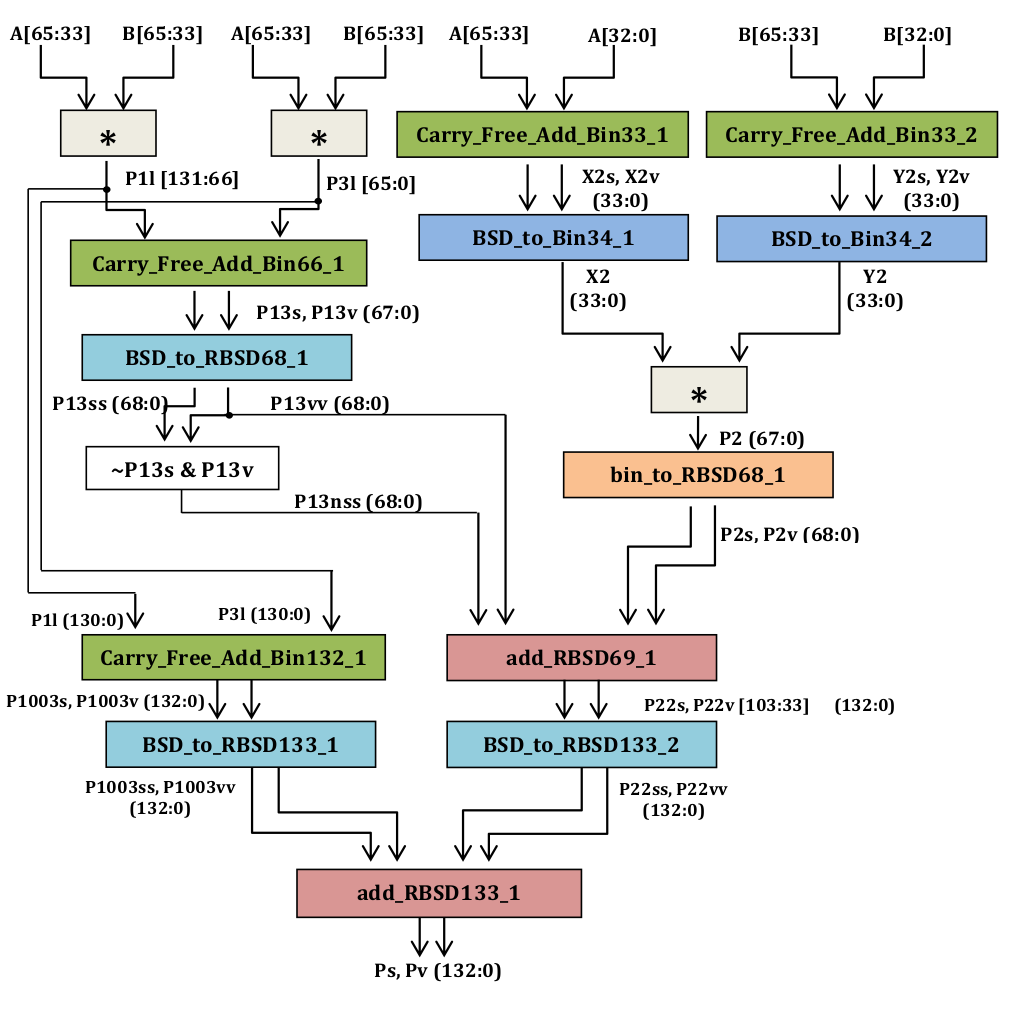
\includegraphics[width=\linewidth]{Mul.png}
\caption{Circuit design of carry-free muliplication of binary numbers.}
\label{fig_sim}
\end{figure}


\section{Results}

All circuits were designed in Verilog and run using Xilinx-9 on a Virtex-5 FPGA (5vlx30ff324). All the modules were also first coded in Octave to verify their computations.

\subsection{Addition}

Table VI lists the comparison of computation times of addition and multiplication between standard implementations and carry-free implementations described in the previous sections. Two metrics were analysed to compare the performance – path delay, Slice Logic Utilization, i.e. the percentage of Slice LUTs on the FPGA utilized, which is equivalent to the Slice Logic Distribution, i.e. the number of LUT Flip-Flop pairs utilized, out of the 19200 present. As can be seen from Table VI, carry-binary binary addition takes lesser memory, as well as significantly lesser time than standard addition.

\vspace{-.5em}
\begin{table}[h!]
  \centering
  \caption{Comparison of Results}
  \label{tab:table6}
  \begin{tabular}{|c|c|c|c|c|}
    \hline
    \textbf{Metric} & \textbf{Standard} & \textbf{Carry-Free} & \textbf{Carry-Free} & \textbf{Carry-Free} \\
    & \textbf{Add} & \textbf{RBSD Add} & \textbf{Binary Add} & \textbf{Mul} \\
    \hline
    \hline
    Path delays & 71.306 ns & 4.784 ns & 4.028 ns & 24.973 ns \\
    \hline
    Slice LUTs & 2\% & 4\% & 1\% & 11\% \\
    \hline
    LUT FF pairs & 384 & 928 & 265 & 2223 \\
    \hline
  \end{tabular}
\end{table}

\subsection{Multiplication}

Table VI also lists the path delay and LUT usage for the carry-free implementation of multiplication. As can be seen, carry-free multiplication takes lesser time than even standard addition, it can be inferred that it takes significantly lesser time than standard multiplication.

\vspace{-.5em}
\begin{table}[h!]
  \centering
  \caption{Path Delays in Carry-Free Multiplication}
  \label{tab:table7}
  \begin{tabular}{|c|c||c|c|}
    \hline
    \textbf{Module} & \textbf{Delay} & BSD\_to\_RBSD68 & 4.028 ns \\
    \hline
    Bin\_to\_RBSD68 & 3.607 ns & BSD\_to\_RBSD132 & 4.028 ns \\
    \hline
    Carry\_Free\_Add\_Bin33 & 4.028 ns & add\_RBSD\_69 & 4.784 ns \\
    \hline
    Carry\_Free\_Add\_Bin66 & 4.028 ns & add\_RBSD\_133 & 4.784 ns \\
    \hline
    Carry\_Free\_Add\_Bin132 & 4.028 ns & BSD\_to\_Bin33 & 12.824 ns \\
    \hline
  \end{tabular}
\end{table}

Table VII lists the path delays of the individual modules in the Carry-Free Multiplier, in ascending order of time taken. It can be observed that the most time-consuming module is the $BSD\_to\_Bin33$ module, which involves carry-full operation. All carry-free operations clearly take less than a third of the time taken by a simple BSD to binary conversion. The advantage of carry-free operation is highlighted in this result.


\section{Analysis}

\subsection{Use of 2’s Complement binary numbers}

Throughout the paper, binary numbers have been assumed to be positive, where $n$-bits of the binary number convert to $2*(n+1)$ bits of the RBSD number ($n+1$ each of sign and value bits). However, negative numbers, i.e. the possible use of binary numbers as being in their 2’s complement forms, has not been explored. The good news here is that this incorporation is particularly easy. In its 2’s complement form, there shall be no increase in number of bits in the binary number's conversion to RBSD, since it already has an extra bit included. If the number is negative, the most significant bit of its RBSD form shall inevitably be -1. Thus, the number of bits would increase to just $2n$.

\subsection{Carry Free Adder combined with BSD-to-RBSD converter}

The field of RBSD numbers is not closed under addition, so the sum of two RBSD numbers, either carry-free or with carry propagation, shall result in a BSD number that is not necessarily RBSD. Since many applications (e.g., computing sums during in multiplication) require further use of the sum, it is imperative to convert the sum into RBSD before using it elsewhere. Fortunately, BSD to RBSD conversion is combinational, so it does not delay the circuit much. This is why every Carry-Free Adder is followed by a BSD-to-RBSD converter in the Carry-Free Multiplier (Figure 2).

It can be argued that a Carry-Free Adder and a BSD-to-RBSD converter should be combined to make one single truth table, so there is no delay in adding RBSD or binary numbers into an RBSD sum. However, making such a concise table is quite painful. The BSD-to-RBSD converter takes 4 consecutive digits of the input BSD number, and produces 1 output digit at the most significant digit position. A Carry-Free Adder takes 2 consecutive digits from each RBSD input, or 3 from each binary input, to produce one output digit at the most significant position. Since these act as inputs to the BSD-to-RBSD Converter, the Carry-Free Adders require 5 consecutive RBSD digits, or 6 consecutive binary bits to produce one output digit at the most significant position. This leads to a table having $3^5 =$ 243 rows in case of RBSD Adder, and $2^6 =$ 64 rows in case of Binary adder. It is practically infeasible, and quite unnecessary, to manually construct a Product-of-Sum form for the combined truth table.

\subsection{Carry-Free Karatsuba Multiplication}

\subsubsection{Multiplication of BSD numbers}

The first step of Karatsuba multiplication involves splitting the input number into two parts. In case of BSD numbers, however, simply splitting the number at the middle is mathematically incorrect, and shall lead to erroneous results. Moreover, mathematically sound splitting involves carry propagation, which opposes our goal of fast computation. So multiplication of BSD numbers is avoided. Instead, the three multiplications in the circuit are of binary numbers (see Figure 1), BSD-to-Binary conversion having explicitly been done in one case for this purpose.

\subsubsection{Carry-full 34-bit BSD-to-Binary converter}

As seen from Table VII, the two 34-bit RBSD-to-Binary converters used in the multiplier (see Figure 1) are the major contributors to the path delay of this circuit, as they involve carry propagation. Unfortunately, it cannot be avoided. If a method is devised that eliminates the need for carry propagation in this conversion, then that method could instead be directly applied in the addition of two numbers.

It could be argued that the use of two 17-bit RBSD-to-Binary converters can help decrease path delay, since they can be run in parallel. However, this would involve splitting the RBSD number which, as discussed above, results in some carry propagation of its own. It is to be seen whether the overall path delay is indeed lesser.

\subsubsection{Multiplication of integers}

Ultimately, multiplication operation is performed using integer arithmetic, which involves carry propagation. It can be argued that the numbers can be split into two 17-bit numbers and integer multiplication can be carried out over them instead of the 34-bit numbers. However, this is equivalent to adding one more level to the Karatsuba multiplication being carried out. This shall result in thrice the number of multiplications involved. It needs to be checked through experimentation whether this incurs lesser delay.

\subsubsection{Multiplication of binary numbers with more than 64 bits}

The original design was meant for 64-bit binary numbers, the extra two bits can be set to 0 to add two $n$-bit numbers, where $n <= 64$. For $n > 64$, each input number could be split into the lowest 64 bits and the rest. The Karatsuba algorithm can then be recursively employed on the two parts.

\section{Conclusion}

It has been quantifiably verified that carry-free implementations of arithmetic operations have significant advantage over standard implementations in terms of path delay and memory. A carry-free multiplier thus designed takes lesser time than standard addition itself. It has been analyzed that the most optimized carry-free implementations are painful to design, so a modular approach of combining Carry-Free Adders to make more complex arithmetic modules is practical.


% An example of a floating figure using the graphicx package.
% Note that \label must occur AFTER (or within) \caption.
% For figures, \caption should occur after the \includegraphics.
% Note that IEEEtran v1.7 and later has special internal code that
% is designed to preserve the operation of \label within \caption
% even when the captionsoff option is in effect. However, because
% of issues like this, it may be the safest practice to put all your
% \label just after \caption rather than within \caption{}.
%
% Reminder: the "draftcls" or "draftclsnofoot", not "draft", class
% option should be used if it is desired that the figures are to be
% displayed while in draft mode.
%
%\begin{figure}[!t]
%\centering
%\includegraphics[width=2.5in]{myfigure}
% where an .eps filename suffix will be assumed under latex, 
% and a .pdf suffix will be assumed for pdflatex; or what has been declared
% via \DeclareGraphicsExtensions.
%\caption{Simulation results for the network.}
%\label{fig_sim}
%\end{figure}

% Note that the IEEE typically puts floats only at the top, even when this
% results in a large percentage of a column being occupied by floats.


% An example of a double column floating figure using two subfigures.
% (The subfig.sty package must be loaded for this to work.)
% The subfigure \label commands are set within each subfloat command,
% and the \label for the overall figure must come after \caption.
% \hfil is used as a separator to get equal spacing.
% Watch out that the combined width of all the subfigures on a 
% line do not exceed the text width or a line break will occur.
%
%\begin{figure*}[!t]
%\centering
%\subfloat[Case I]{\includegraphics[width=2.5in]{box}%
%\label{fig_first_case}}
%\hfil
%\subfloat[Case II]{\includegraphics[width=2.5in]{box}%
%\label{fig_second_case}}
%\caption{Simulation results for the network.}
%\label{fig_sim}
%\end{figure*}
%
% Note that often IEEE papers with subfigures do not employ subfigure
% captions (using the optional argument to \subfloat[]), but instead will
% reference/describe all of them (a), (b), etc., within the main caption.
% Be aware that for subfig.sty to generate the (a), (b), etc., subfigure
% labels, the optional argument to \subfloat must be present. If a
% subcaption is not desired, just leave its contents blank,
% e.g., \subfloat[].


% An example of a floating table. Note that, for IEEE style tables, the
% \caption command should come BEFORE the table and, given that table
% captions serve much like titles, are usually capitalized except for words
% such as a, an, and, as, at, but, by, for, in, nor, of, on, or, the, to
% and up, which are usually not capitalized unless they are the first or
% last word of the caption. Table text will default to \footnotesize as
% the IEEE normally uses this smaller font for tables.
% The \label must come after \caption as always.
%
%\begin{table}[!t]
%% increase table row spacing, adjust to taste
%\renewcommand{\arraystretch}{1.3}
% if using array.sty, it might be a good idea to tweak the value of
% \extrarowheight as needed to properly center the text within the cells
%\caption{An Example of a Table}
%\label{table_example}
%\centering
%% Some packages, such as MDW tools, offer better commands for making tables
%% than the plain LaTeX2e tabular which is used here.
%\begin{tabular}{|c||c|}
%\hline
%One & Two\\
%\hline
%Three & Four\\
%\hline
%\end{tabular}
%\end{table}


% Note that the IEEE does not put floats in the very first column
% - or typically anywhere on the first page for that matter. Also,
% in-text middle ("here") positioning is typically not used, but it
% is allowed and encouraged for Computer Society conferences (but
% not Computer Society journals). Most IEEE journals/conferences use
% top floats exclusively. 
% Note that, LaTeX2e, unlike IEEE journals/conferences, places
% footnotes above bottom floats. This can be corrected via the
% \fnbelowfloat command of the stfloats package.

% conference papers do not normally have an appendix


% use section* for acknowledgment
\section*{Acknowledgment}


The author would like to thank Sujoy Sinha Roy and Prof. Ingrid Verbauwhede from KU Leuven, Belgium, for the opportunity to collaborate with them on this work.


% trigger a \newpage just before the given reference
% number - used to balance the columns on the last page
% adjust value as needed - may need to be readjusted if
% the document is modified later
%\IEEEtriggeratref{8}
% The "triggered" command can be changed if desired:
%\IEEEtriggercmd{\enlargethispage{-5in}}

% references section

% can use a bibliography generated by BibTeX as a .bbl file
% BibTeX documentation can be easily obtained at:
% http://mirror.ctan.org/biblio/bibtex/contrib/doc/
% The IEEEtran BibTeX style support page is at:
% http://www.michaelshell.org/tex/ieeetran/bibtex/
%\bibliographystyle{IEEEtran}
% argument is your BibTeX string definitions and bibliography database(s)
%\bibliography{IEEEabrv,../bib/paper}
%
% <OR> manually copy in the resultant .bbl file
% set second argument of \begin to the number of references
% (used to reserve space for the reference number labels box)
\begin{thebibliography}{1}

\bibitem{IEEEhowto:kopka}
P.~Kogge and H.~Stone, \emph{A parallel algorithm for the efficient solution of a general class of recurrences}, IEEE Transactions on Computers (T-C), vol. 22, pp. 786-793, 1973.

\bibitem{IEEEhowto:kopka}
B.~Parhami, \emph{Computer Arithmetic - Algorithms and Hardware Designs}. Oxford University Press, 2000.

\bibitem{IEEEhowto:kopka}
A.~Avizienis, \emph{Signed-digit number representations for fast parallel arithmetic}, IRE Transactions on Electronic Computers, vol. 10, no. 3, pp. 389-400, 1961.

\bibitem{IEEEhowto:kopka}
B.~Parhami, \emph{Generalized signed-digit number systems: A unifying framework for redundant number representations}, IEEE Transactions on Computers (T-C), vol. 39, no. 1, pp.  89-98, 1990.

\bibitem{IEEEhowto:kopka}
F.~Kharbash, G.~M.~Chaudhry, \emph{Reliable Binary Signed Digit Number Adder Design}, IEEE Computer Society Annual Symposium on VLSI, pp 479-484, 2007.

\bibitem{IEEEhowto:kopka}
J.~Moskal, E.~Oruklu and J.~Saniie, \emph{Design and Synthesis of a Carry-Free  Signed-Digit Decimal Adder}, IEEE International symposium on Circuits and Systems, pp. 1089-1092, 2007.

\bibitem{IEEEhowto:kopka}
R.~Rani, N.~Sharma, L.~K.~Singh, \emph{Fast Computing using Signed Digit Number System}, IEEE proceedings of International Conference on Control, Automation, Communication And  Energy Conservation, 2009.

\bibitem{IEEEhowto:kopka}
K.~Schneider, A.~Willenbucher, \emph{A New Algorithm for Carry-Free Addition of Binary Signed-Digit Numbers}, IEEE 22nd International Symp. Field-Programmable Custom Computing Machines, 2014.

\bibitem{IEEEhowto:kopka}
B.~Parhami, \emph{Carry-free addition of recoded binary signed-digit numbers}, IEEE Transactions on Computers (T-C), vol. 37, no. 11, pp. 1470-1476, 1998.

\bibitem{IEEEhowto:kopka}
M.~Joye and S.~M.~Yen, \emph{Optimal left-to-right binary signed-digit recoding}, IEEE Transactions on Computers (T-C), vol. 49, no. 7, pp. 740-748, 2000.

\bibitem{IEEEhowto:kopka}
J.~U.~Ahmed, A.~A.~S.~Awwal, \emph{Multiplier design using RBSD number system}, Proceedings of the 1993 National Aerospace and Electronics Conference, vol. 1, pp. 180-184, 1993.

\bibitem{IEEEhowto:kopka}
A.~K.~Cherri, M.~S.~Alam, \emph{Recoded and nonrecoded trinary signed-digit multipliers designs using redundant bit representations}, Aerospace and Electronics Conference 1998. NAECON 1998. Proceedings of the IEEE 1998 National, pp. 505-512, 1998, ISSN 0547-3578, 1998.

\bibitem{IEEEhowto:kopka}
T.~N.~Rajashekhar and O.~Kal, \emph{Fast Multiplier Design using Redundant Signed-Digit Numbers}, International Journal of Electronics, vol .69, no. 3, pp. 359-368, 1990.

\bibitem{IEEEhowto:kopka}
A.~Karatsuba and Y.~Ofman, \emph{Multiplication of Many-Digital Numbers by Automatic Computers}, Proceedings of the USSR Academy of Sciences. 145: 293-294. Translation in the academic journal Physics-Doklady, 7 (1963), pp. 595-596, 1962.

\bibitem{IEEEhowto:kopka}
A.~A.~S.~Awwal and J.~U.~Ahmed, \emph{Fast carry free adder design using QSD number system}, Proceedings of the IEEE 1993 National Aerospace and Electronic Conference, vol 2, pp. 1085-1090, 1993.

\bibitem{IEEEhowto:kopka}
R.~Rani, L.~K.~Singh and N.~Sharma, \emph{A Novel design of High Speed Adders Using Quaternary Signed Digit Number System}, International Journal of Computer and Network Security (IJCNS), Vol. 2, No. 9, pp. 62-66, 2010.

\bibitem{IEEEhowto:kopka}
N.~W.~Umredkar, M.~A.~Gaikwad, \emph{Review of Quaternary Adders in Voltage Mode  Multi-Valued Logic}, International Journal of Computer Applications (0975–8887), 2013.

% \bibitem{IEEEhowto:kopka}
% S.~Dubey, R.~Rani, \emph{VLSI Implementation of Fast Addition using Quaternary Signed Digit Number System}, IEEE International Conference on Emerging Trends in  Comp...ICECCN 2013.

\bibitem{IEEEhowto:kopka}
O.~Ishizuka, A.~Ohta, K.~Tannno, Z.~Tang, D.~Handoko, \emph{VLSI design of a quaternary multiplier with direct generation of partial products}, Proceedings of the 27th International Symposium on Multiple-Valued Logic, pp. 169-174, 1997.

\bibitem{IEEEhowto:kopka}
S.~Datla and M.~Thornton, \emph{Quaternary Voltage-Mode Logic Cells and Fixed-Point Multiplication Circuits}, Multiple-Valued Logic (ISMVL) 2010 40th IEEE  International Symposium on, pp. 128-133, 2010, ISSN 0195-623X, 2010.

\bibitem{IEEEhowto:kopka}
N.~Sharma, B.~S.~Rai and A.~Kumar, \emph{Design of RBSD Adder and Multiplier Circuits for High Speed Arithmetic Operations and Their Timing Analysis}, Special Russian Issue: Advances in Computer Science and Engineering, Research in Computing Science, pp. 243-25, 2006.

\end{thebibliography}


% that's all folks
\end{document}
